\section{Auswertung}
\label{sec:Auswertung}
\subsection{Mittlere Weglänge}

Um die mittlere Weglänge $\bar{w}$ der Elektronen zu bestimmen werden die Gleichungen
\ref{eqn:wegl} und \ref{eqn:psat} genutzt. Die berechneten Werte sind in Tabelle
\ref{tab:tab1} zu finden. Die mittlere Weglänge $\bar{w}$ wird mit dem Abstand
$a=\SI{1e-2}{\m}$ zwischen
Kathode und Beschleunigungselektrode verglichen.

\begin{table}[H]
  \centering
  \caption{Messwerte zur Bestimmung der RC-Konstanten}
  \label{tab:tabe1}
    \begin{tabular}{c c c c}
    \toprule
    $ t \: / \si{\milli\second} $ & $ U_C \: / \si {\volt} $ & $\frac{U_C}{U_0} $
    & $ \ln{\frac{U_C}{U_0}} $ \\
    \midrule
    0.000 & 12.00 & 1.000 & 0.000 \\
    0.080 & 10.88 & 0.907 & -0.098 \\
    0.160 & 9.84 & 0.820 & -0.198 \\
    0.240 & 8.96 & 0.747 & -0.292 \\
    0.320 & 8.16 & 0.680 & -0.386 \\
    0.400 & 7.44 & 0.620 & -0.478 \\
    0.480 & 6.80 & 0.567 & -0.568 \\
    0.560 & 6.16 & 0.513 & -0.667 \\
    0.640 & 5.68 & 0.473 & -0.748 \\
    0.720 & 5.20 & 0.433 & -0.836 \\
    0.800 & 4.72 & 0.393 & -0.933 \\
    0.880 & 4.32 & 0.360 & -1.022 \\
    0.960 & 4.00 & 0.333 & -1.099 \\
    1.040 & 3.68 & 0.307 & -1.182 \\
    1.120 & 3.36 & 0.280 & -1.273 \\
    1.200 & 3.12 & 0.260 & -1.347 \\
    1.280 & 2.88 & 0.240 & -1.427 \\
    1.360 & 2.64 & 0.220 & -1.514 \\
    1.440 & 2.48 & 0.207 & -1.577 \\
    1.520 & 2.32 & 0.193 & -1.643 \\
    1.600 & 2.16 & 0.180 & -1.715 \\
    1.680 & 2.00 & 0.167 & -1.792 \\
    1.760 & 2.00 & 0.167 & -1.792 \\

      \bottomrule
    \end{tabular}
\end{table}


\subsection{Differentielle Energieverteilung}
Hier werden die Graphen 1 und 2 aus dem Anhang verwendet.
Zunächst wird aus der Skalierung der x-Achse ermittelt, wie viele
Skalenteile einem Volt entsprechen. Dazu werden die Skalenteile zwischen einer
Markierung (entspricht einem Volt) abgezählt, die Ergebnisse sind in
Tabelle \ref{tab:tab2} zu sehen. Da auf Millimeterpapier gezeichnet wird entspricht
ein Skalenteil einem Millimeter.

\begin{table}[H]
  \centering
  \caption{Amplitude in Abhängigkeit der Frequenz}
  \label{tab:tabe2}
    \begin{tabular}{c c}
    \toprule
    $ \nu \: / \si{\hertz} $ & $ U_C \: / \si {\volt} $ \\
    \midrule
    10 & 14.85 \\
    30 & 14.65 \\
    70 & 13.94 \\
    100 & 13.15 \\
    300 & 8.40 \\
    700 & 4.28 \\
    1000 & 3.09 \\
    2000 & 1.50 \\
    3000 & 1.01 \\
    4000 & 0.76 \\
    5000 & 0.62 \\

    \bottomrule
    \end{tabular}
\end{table}

Da der Abstand zwischen zwei Markierungen einem Volt entspricht wird der
Kehrwert der Mittelwerte gebildet:
\begin{align*}
  V_1=\SI{0,041(1)}{\V}\\
  V_2=\SI{0,042(1)}{\V}.
\end{align*}
Um aus der integralen
Energieverteilung die differentielle Energieverteilung zu erhalten, werden
Steigungsdreiecke eingezeichnet. Die Abgelesenen Steigungen, sowie
die dazugehörigen Werte der Bremsspannung stehen in Tabelle \ref{tab:tab3}.

\begin{table}[H]
  \centering
  \caption{Phasenverschiebung in Abhängigkeit der Frequenz}
  \label{tab:tabe3}
    \begin{tabular}{c c c c}
    \toprule
    $ \nu \: / \si{\hertz} $ & $ a \: / \si {\milli \second} $ & $ b \:
     / \: \si{\milli \second} $
    & $ \phi \: / \: rad $ \\
    \midrule
    10 & 0.40 & 100.00 & 0.025 \\
    30 & 0.80 & 33.33 & 0.151 \\
    70 & 0.80 & 14.29 & 0.352 \\
    100 & 0.88 & 10.00 & 0.553\\
    300 & 0.48 & 3.33 & 0.906\\
    700 & 0.28 & 1.43 & 1.230\\
    1000 & 0.22 & 1.00 & 1.382\\
    2000 & 0.11 & 0.50 & 1.382\\
    3000 & 0.08 & 0.33 & 1.523\\
    4000 & 0.06 & 0.25 & 1.508\\
    5000 & 0.05 & 0.20 & 1.571\\

      \bottomrule
    \end{tabular}
\end{table}


In Abbildung \ref{fig:plot1} und \ref{fig:plot2} wird
diese Steigung gegen die Bremsspannung $U_A$ aufgetragen. Dabei ist zu beachten, dass
die Steigung proportional zu Anzahl der Elektronen ist, während die Bremsspannung $U_A$
ein Maß für die Energie der Elektronen ist.


\begin{figure}[H]
  \centering
  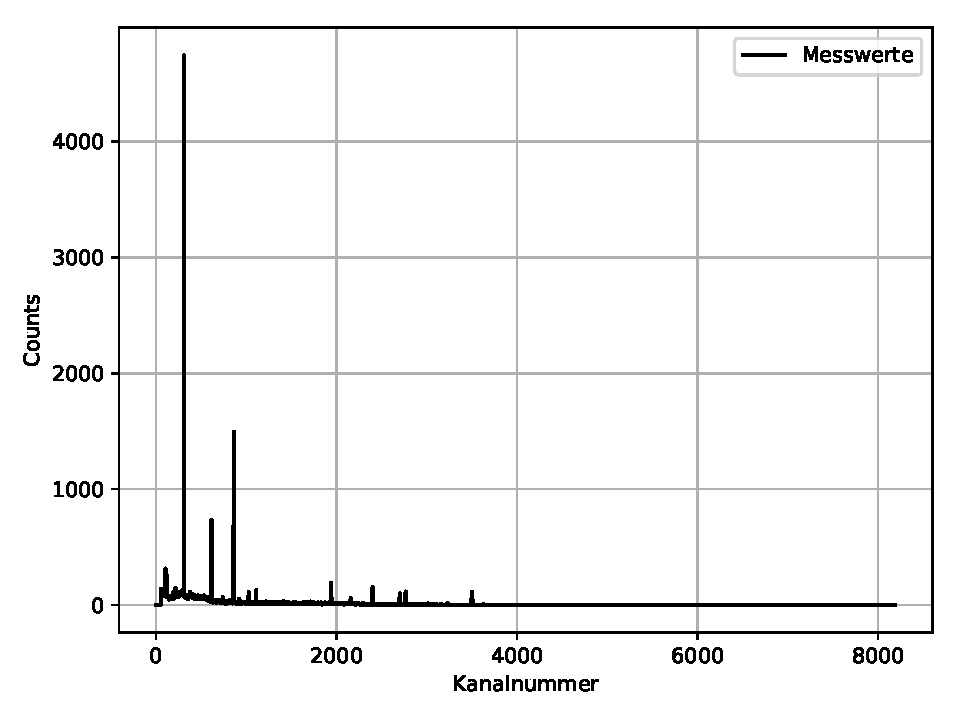
\includegraphics[height=7cm]{plot1.pdf}
  \caption{Differentielle Energieverteilung bei 300\;K }
  \label{fig:plot1}
\end{figure}

 \begin{figure}[H]
   \centering
   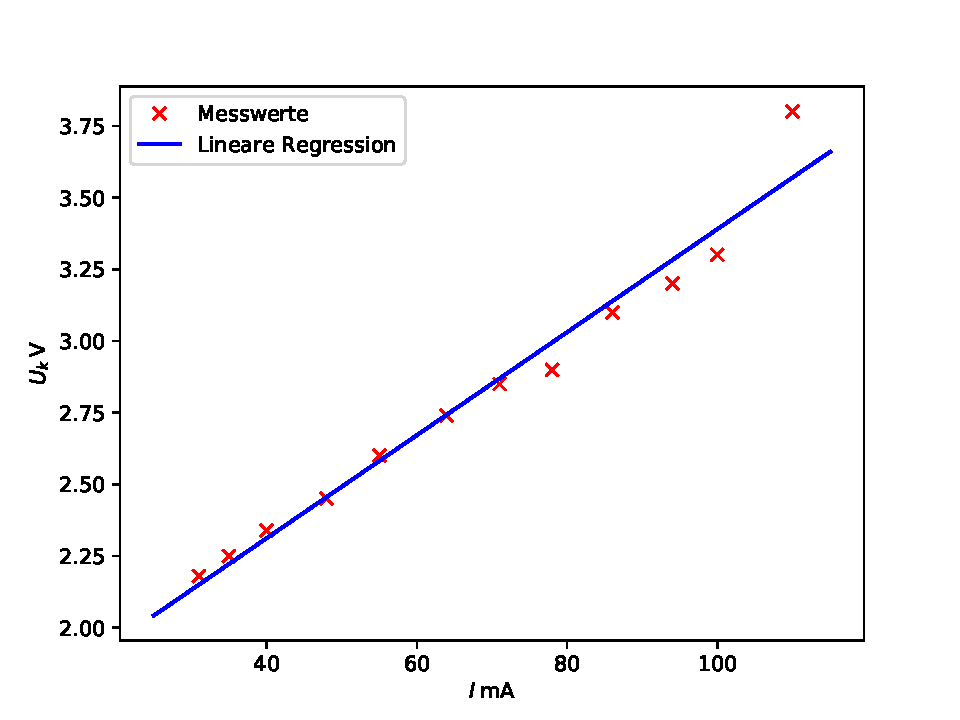
\includegraphics[height=7cm]{plot2.pdf}
   \caption{Differentielle Energieverteilung bei 422\;K}
   \label{fig:plot2}
 \end{figure}

Aus Abbildung \ref{fig:plot1} lässt sich ablesen, dass die meisten Elektronen
die Energie $E=\SI{6,73}{\eV}$ besitzen.
Da eine Beschleunigungsspannung von $U_B=\SI{11}{V}$ angelegt wurde berechnet sich das
Kontaktpotential nach Formel \ref{eqn:kontaktpotential} wie folgt:
\begin{equation}
  K=\frac{1}{e_0}(\SI{6,73}{\eV})=\SI{6,73}{\V}.
  \label{kontakt}
\end{equation}
Daraus ergibt sich das effektive Beschleunigungspotential:
\begin{equation}
  U_{\text{B,eff}}= U_B -K =\SI{4,27}{\V}.
\end{equation}

Zwischen Abbildung \ref{fig:plot1} und \ref{fig:plot2} ist ein deutlicher
Unterschied zu erkennen. Das lässt sich über die freie Weglänge, bzw. das Verhältnis
$\frac{a}{\bar{w}}$ erklären. Bei Zimmertemperatur ist der Gasdruck deutlich geringer,
also ist die freie Weglänge größer und damit das Verhältnis $\frac{a}{\bar{w}}$
kleiner. Also stoßen die Elektronen nicht so häufig gegen Hg-Atome. Das ist bei der zweiten
Messreihe schon deutlich öfter der Fall und da die Elektronen bei jedem Stoß ihre
Richtung und Geschwindigkeit ändern, kommt es zu einer breiteren Energieverteilung
an der Anode.
%Einbruch bei ca. 2,5V

\subsection{Frank-Hertz-Kurve}
Hier wird zu Beginn ebenfalls über die Skalierung der x-Achse ermittelt wie viele
Skalenteile einem Volt entsprechen.
\begin{table}[H]
  \centering
   \begin{tabular}{c c c c }
    \toprule
    $\Delta U$ & Skalenteile (T=466\;K) & Skalenteile (T=437\;K) &  Skalenteile (T=446\;K)\\
    \midrule
    0-5 & 23 & 19 & 17\\
    5-10 & 20 & 20 & 20\\
    10-15 & 20 &20 & 22\\
    15-20 & 20& 20& 19\\
    20-25 & 22& 23 & 22\\
    25-30 & 22 & 20 & 20\\
    30-35 & 21 & 20 & 21\\
    35-40 & 20 & 22 & 21\\
    40-45 & 20 & 20 & 26\\
    45-50 & 21 & 20 & 17\\
    50-55 & 21 & 22 & 20\\

    \midrule
    $\implies$& $\SI{20,91(31)}{}$ & $\SI{20,55(37)}{}$ & $\SI{20,45(76)}{}$\\
    \bottomrule
  \end{tabular}
  \caption{Werte zur Skalierung der x-Achse.}
  \label{tab:tab4}
\end{table}
%V3=0,239
%V4=0,243
%V5=0,244

Hier wurden die Markierungen in Abständen von $\SI{5}{\V}$ gemacht, somit ergibt
sich aus den Mittelwerten der Skaleneinheiten:
\begin{align*}
  V3=\SI{0,239(4)}{\V}\\
  V4=\SI{0,243(4)}{\V}\\
  V5=\SI{0,244(9)}{\V}.
\end{align*}
Um die erste Anregungsenergie $E_1$ zu bestimmen werden die Abstände zwischen den
Maxima von Anhang 3-5 gemessen, dies ist in Tabelle \ref{tab:tab5} zu sehen.
Denn der Abstand zwischen den Maxima multipliziert mit
$e_0$ entspricht der ersten Anregungsenergie.
\begin{table}[H]
  \centering
   \begin{tabular}{c c c c }
    \toprule
    $\Delta U$ & $U_{k+1}-U_K$/Skt (T=466\;K) & $U_{k+1}-U_K$/Skt (T=437\;K) & $U_{k+1}-U_K$/Skt (T=446\;K) \\
    \midrule
    1 & 18 & 19 & 20\\
    2 & 20 & 20 & 19\\
    3 & 21 & 20 & 20\\
    4 & 21 & 22 & 20\\
    5 & 21 & 23 & 20\\
    6 & 22 &    & 21\\
    7 & 22 &    & 22\\
    8 & 22 &    & 21\\
    \midrule
    $\implies$& $\SI{20.88(48)}{}$ & $\SI{20.8(7)}{}$ &  $\SI{20.38(32)}{}$\\
    \bottomrule
  \end{tabular}
  \caption{Abstände zwischen den Maxima der Frank-Hertz-Kurve.}
  \label{tab:tab5}
\end{table}

Die Abstände der Maxima umgerechnet in Volt ergeben:
\begin{align*}
  V_{3,A}=\SI{4,99(14)}{\V}\\
  V_{4,A}=\SI{5,05(20)}{\V}\\
  V_{5,A}=\SI{4,97(20)}{\V}.
\end{align*}

So ergibt sich der Mittelwert für die erste Anregungsenergie $E_1$:
\begin{align*}
  E_1=\SI{5,01(10)}{\eV}.
\end{align*}

Mit der Beziehung $\lambda=\frac{c}{\nu}$ und $E=h\nu$ ergibt sich für die Wellenlänge
\begin{equation}
  \lambda=\SI{247(5)}{\nm}.
\end{equation}

\subsection{Ionisierungsenergie}
Um die Ionisierungsenergie zu ermitteln wird in Anhang 6 eine Asymptote eingezeichnet,
diese schneidet die x-Achse bei $X=\SI{15,2}{\V}$.
Mit dem Kontaktpotential, dass schon in Rechnung \ref{kontakt} bestimmt
wurde ergibt sich:
\begin{equation}
  U_{\text{Ionisierung}}=(X-K)\cdot e_0=\SI{8,47}{\eV}.
\end{equation}
